

%% This file was auto-generated by IPython.
%% Conversion from the original notebook file:
%%
\documentclass[11pt,english]{article}

%% This is the automatic preamble used by IPython.  Note that it does *not*
%% include a documentclass declaration, that is added at runtime to the overall
%% document.

\usepackage{amsmath}
\usepackage{amssymb}
\usepackage{graphicx}
\usepackage{grffile}
\usepackage{ucs}
\usepackage[utf8x]{inputenc}

% Scale down larger images
\usepackage[export]{adjustbox}

%fancy verbatim
\usepackage{fancyvrb}
% needed for markdown enumerations to work
\usepackage{enumerate}

% Slightly bigger margins than the latex defaults
\usepackage{geometry}
\geometry{verbose,tmargin=3cm,bmargin=3cm,lmargin=2.5cm,rmargin=2.5cm}

% Define a few colors for use in code, links and cell shading
\usepackage{color}
\definecolor{orange}{cmyk}{0,0.4,0.8,0.2}
\definecolor{darkorange}{rgb}{.71,0.21,0.01}
\definecolor{darkgreen}{rgb}{.12,.54,.11}
\definecolor{myteal}{rgb}{.26, .44, .56}
\definecolor{gray}{gray}{0.45}
\definecolor{lightgray}{gray}{.95}
\definecolor{mediumgray}{gray}{.8}
\definecolor{inputbackground}{rgb}{.95, .95, .85}
\definecolor{outputbackground}{rgb}{.95, .95, .95}
\definecolor{traceback}{rgb}{1, .95, .95}

% new ansi colors
\definecolor{brown}{rgb}{0.54,0.27,0.07}
\definecolor{purple}{rgb}{0.5,0.0,0.5}
\definecolor{darkgray}{gray}{0.25}
\definecolor{lightred}{rgb}{1.0,0.39,0.28}
\definecolor{lightgreen}{rgb}{0.48,0.99,0.0}
\definecolor{lightblue}{rgb}{0.53,0.81,0.92}
\definecolor{lightpurple}{rgb}{0.87,0.63,0.87}
\definecolor{lightcyan}{rgb}{0.5,1.0,0.83}

% Framed environments for code cells (inputs, outputs, errors, ...).  The
% various uses of \unskip (or not) at the end were fine-tuned by hand, so don't
% randomly change them unless you're sure of the effect it will have.
\usepackage{framed}

% remove extraneous vertical space in boxes
\setlength\fboxsep{0pt}

% codecell is the whole input+output set of blocks that a Code cell can
% generate.

% TODO: unfortunately, it seems that using a framed codecell environment breaks
% the ability of the frames inside of it to be broken across pages.  This
% causes at least the problem of having lots of empty space at the bottom of
% pages as new frames are moved to the next page, and if a single frame is too
% long to fit on a page, will completely stop latex from compiling the
% document.  So unless we figure out a solution to this, we'll have to instead
% leave the codecell env. as empty.  I'm keeping the original codecell
% definition here (a thin vertical bar) for reference, in case we find a
% solution to the page break issue.

%% \newenvironment{codecell}{%
%%     \def\FrameCommand{\color{mediumgray} \vrule width 1pt \hspace{5pt}}%
%%    \MakeFramed{\vspace{-0.5em}}}
%%  {\unskip\endMakeFramed}

% For now, make this a no-op...
\newenvironment{codecell}{}

 \newenvironment{codeinput}{%
   \def\FrameCommand{\colorbox{inputbackground}}%
   \MakeFramed{\advance\hsize-\width \FrameRestore}}
 {\unskip\endMakeFramed}

\newenvironment{codeoutput}{%
   \def\FrameCommand{\colorbox{outputbackground}}%
   \vspace{-1.4em}
   \MakeFramed{\advance\hsize-\width \FrameRestore}}
 {\unskip\medskip\endMakeFramed}

\newenvironment{traceback}{%
   \def\FrameCommand{\colorbox{traceback}}%
   \MakeFramed{\advance\hsize-\width \FrameRestore}}
 {\endMakeFramed}

% Use and configure listings package for nicely formatted code
\usepackage{listingsutf8}
\lstset{
  language=python,
  inputencoding=utf8x,
  extendedchars=\true,
  aboveskip=\smallskipamount,
  belowskip=\smallskipamount,
  xleftmargin=2mm,
  breaklines=true,
  basicstyle=\small \ttfamily,
  showstringspaces=false,
  keywordstyle=\color{blue}\bfseries,
  commentstyle=\color{myteal},
  stringstyle=\color{darkgreen},
  identifierstyle=\color{darkorange},
  columns=fullflexible,  % tighter character kerning, like verb
}

% The hyperref package gives us a pdf with properly built
% internal navigation ('pdf bookmarks' for the table of contents,
% internal cross-reference links, web links for URLs, etc.)
\usepackage{hyperref}
\hypersetup{
  breaklinks=true,  % so long urls are correctly broken across lines
  colorlinks=true,
  urlcolor=blue,
  linkcolor=darkorange,
  citecolor=darkgreen,
  }

% hardcode size of all verbatim environments to be a bit smaller
\makeatletter 
\g@addto@macro\@verbatim\small\topsep=0.5em\partopsep=0pt
\makeatother 

% Prevent overflowing lines due to urls and other hard-to-break entities.
\sloppy




\begin{document}




\section{{[}WS13/14{]} Mathematics for Robotics and Control Assignment
008 - Control}


\begin{codecell}


\begin{codeinput}
\begin{lstlisting}
import IPython.core.display
import sys
if not "win" in sys.platform and not "linux" in sys.platform:
    %pylab
else:
    %pylab inline
\end{lstlisting}
\end{codeinput}
\begin{codeoutput}


\begin{Verbatim}[commandchars=\\\{\}]
Populating the interactive namespace from numpy and matplotlib
\end{Verbatim}

\end{codeoutput}

\end{codecell}

\begin{codecell}


\begin{codeinput}
\begin{lstlisting}
import sympy

s = sympy.Symbol("s")
\end{lstlisting}
\end{codeinput}

\end{codecell}

\begin{center}\rule{3in}{0.4pt}\end{center}

\subsubsection{Assignment 8.1 {[}L1{]}}


Answer the following questions:

\begin{enumerate}[1.]
\item
  What is open-loop control?
\item
  What is closed-loop control?
\item
  What is a transfer function?
\item
  What is the difference between the open and closed transfer function?
\item
  What are poles, what are zeros of a transfer function?
\item
  Given that the numerator and denominator polynomials of a transfer
  function have real coefficients, what does that mean for the poles of
  the transfer function (mathematically)? What does it mean for the
  zeros?
\item
  What is the order of a system? How can you determine it, given the
  different system representations you know?
\item
  Imagine you have a system description made up of several ODEs, how
  would you obtain a system representation that you can easily
  analyze/simulate/control on a computer?
\item
  What is the steady-state response of a system?
\item
  What is the transient response of a system?
\item
  What is the homogenuous response of a system?
\item
  What is the step response of a system?
\item
  What is the impulse response of a system?
\item
  For each response, describe it's usefulness / applications. Why are we
  interested in the different responses? What do they tell us?
\item
  Describe the transient response and it's importance in your own words.
\item
  What are the properties of the transient response? How can you
  determine each of the properties given a system's description?
\end{enumerate}

\section{Solution 8.1}

\begin{enumerate}[1.]
\item
  An open loop control does not have a feedback
\item
  A closed-loop control does have a feedback to the input
\item
  The transfer function is the mathematic representation of a control
  loop
\item
  The closed loop transfer function has G(s) in H(s). (A Feedback)
\item
  At a pole th tranfer function approaches infinity ((H(s) = 0) At a
  zero position the transfer function approaches 0.(H(s) = G(s))
\item
  The zero is where the denominator is equals to the numerator. The pole
  is where the denominator is zero.
\item
  The order of a system is the number of independen enegy storage elemnt
  in the system (Spring, damper\ldots{}). In partial fraction expansion
  this is the number of all Ss, in the diff. eq. it is the highest
  exponent.
\item
  Obtain the tranfer functions of the ODEs and convert them into a
  single transfer function.
\item
  The steady state response is the respons a system may converge into if
  the input does not change.
\item
  The transient response describes how to system will converge. It may
  be over- or underdamped, or even oscillating.
\item
  A system has a homogeneous response if the output with input i and
  i\emph{x is o and o}x
\item
  The step response is the system response after one (n) time steps of
  the system. If the system runs at 1 hz, the first step resonse will be
  the value after 1 second.
\item
  The impulse response the the systems response to an impulse signal.
  14.overdamped: the function is approaching the steady state really
  slow. It is usefull for systems that are not timecritical. Eg. a
  floodgate.
\end{enumerate}
underdamped: the function is approaching the steady state quite fast but
overshoots It is useful for a system that physically can not overshoot
or if we do not care. Like a swing door.

undamped: the function does not approach the steady state. This is not
very useful, except as a generator, like a pendulum clock.

critically damped: the function is approaching the steady state as fast
as possible without overshooting. This often is the desired system.It
does not overshoot and is quite fast. Like a door closer. 15. The
transient respond it the behaviour of the system it will show until it
reaches the steady state. It is important because it may be of
importance because we want to tweak the peak(Overshoot or not), the time
until we reach it or the steady state and how close we get to the steady
state(Steady state error). 16. Overshooting: If and how much the system
will get over the steady state. Settling time: The time needed to reach
and stay at the steady state (within a given acceptance). Peak time: At
which time is the first peak reached. Steady State Error: The difference
between the steady state and the desired state.

\emph{Assignment 8.1 took me} \emph{minutes.}

\begin{center}\rule{3in}{0.4pt}\end{center}

\subsubsection{Assignment 8.2 {[}L1{]}}


The archive uploaded during the last lab class contains a file
\textbf{Control 1.pdf}. From that slide set, page 18, you know that
given a transfer function

$H(s) = \frac{1}{(s+a) \cdot (s+b) \cdot (s+c)}$

you can decompose the denominator into

$H(s) = \frac{K_1}{(s+a)} + \frac{K_2}{(s+b)} + \frac{K_3}{(s+c)}$

for some gain values $K_1, K_2$ and $K_3$, using partial fraction
expansion. This was also covered in the lecture on the Laplace transform
given by your fellow student last week.

\begin{enumerate}[1.]
\item
  Apply the inverse Laplace transformation to each of the components
  factored out in the example above. What is the result?
\item
  What are $a$, $b$ and $c$ in the example above, i.e.~what is their
  type?
\item
  You know by now that the transfer function $H(s)$ characterizes the
  behavior of a system. How do components such as those given in the
  example above influence the behavior of the system? What can you tell
  about each component given the values for $a$, $b$ and $c$? How does
  the range of each value for $a$, $b$ and $c$ influence the component?
\item
  What influence does each $K$ have?
\end{enumerate}

\begin{codecell}


\begin{codeinput}
\begin{lstlisting}
#1
from sympy.integrals import inverse_laplace_transform
a, b, c, s, t, K1, K2, K3 = sympy.symbols('a b c s t K1 K2 K3')

H = sympy.Function('H')(s)
fun = sympy.Eq(H, (K1/(s+a))+(K2/(s+b))+(K3/(s+c)))

sympy.pprint(inverse_laplace_transform(K1/(s+a), s, t))
sympy.pprint(inverse_laplace_transform(K2/(s+b), s, t))
sympy.pprint(inverse_laplace_transform(K3/(s+c), s, t))
\end{lstlisting}
\end{codeinput}
\begin{codeoutput}


\begin{Verbatim}[commandchars=\\\{\}]
-t*re(a)  -i*t*im(a)             
K1*e        *e          *Heaviside(t)
    -t*re(b)  -i*t*im(b)             
K2*e        *e          *Heaviside(t)
    -t*re(c)  -i*t*im(c)             
K3*e        *e          *Heaviside(t)
\end{Verbatim}

\end{codeoutput}

\end{codecell}

# 2. They are complex numbers (real and imaginary part)
# 3. K is the gain, a, b, c are the poles
# 4. K influences the factor by which the input values gets in/decreased.

\emph{Assignment 8.2 took me} \emph{minutes.}

\begin{center}\rule{3in}{0.4pt}\end{center}

\subsubsection{Assignment 8.3 {[}L1{]}}


Assume you are given a transfer function

$H(s) = \frac{2 \cdot s + 1}{s^2 + 3 \cdot s + 2}$

Partial fraction expansion yields:
$H(s) = -\frac{1}{s+1} + \frac{3}{s+2}$

Now, you want to obtain a pole-zero plot of the transfer function in
order to evaluate the underlying system's properties. Using the Python
control library you installed in a previous assignment, we can do the
following. Note how the coefficients are used to create a transfer
function:

\begin{codecell}


\begin{codeinput}
\begin{lstlisting}
import control
tf = control.tf( [2, 1], [1, 3, 2])
print tf
\end{lstlisting}
\end{codeinput}
\begin{codeoutput}


\begin{Verbatim}[commandchars=\\\{\}]
2 s + 1
-------------
s^2 + 3 s + 2
\end{Verbatim}

\end{codeoutput}

\end{codecell}

Now, obtain a pole/zero plot of the transfer function:

\begin{codecell}


\begin{codeinput}
\begin{lstlisting}
control.pzmap.pzmap(tf)
\end{lstlisting}
\end{codeinput}
\begin{codeoutput}




\begin{verbatim}
(array([-2., -1.]), array([-0.5]))
\end{verbatim}



\begin{center}
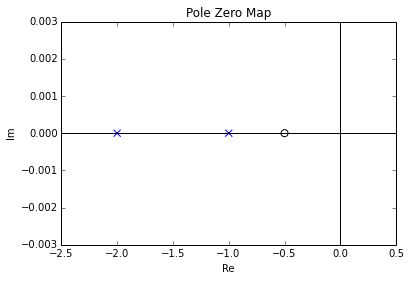
\includegraphics[max size={0.7\textwidth}{0.9\textheight}]{MRC_QUIGNONCHRISTOPHE_20140602_files/MRC_QUIGNONCHRISTOPHE_20140602_22_1.png}
\par
\end{center}

\end{codeoutput}

\end{codecell}

\textbf{Factor the transfer functions denominator and compare the result
with the plot above. Is the result as you would expect? Discuss.}

\begin{codecell}


\begin{codeinput}
\begin{lstlisting}
denominator = s**2 + 3*s + 2
sympy.pretty_print( sympy.factor(denominator) )
\end{lstlisting}
\end{codeinput}
\begin{codeoutput}


\begin{Verbatim}[commandchars=\\\{\}]
(s + 1)*(s + 2)
\end{Verbatim}

\end{codeoutput}

\end{codecell}
\paragraph{Answer 8.3.1}


# The result is as expected.
# The root is where the function aproaches infinity, which is when the denominator = 0, which is if one of terms of the factorized denominator is zero:
# (s + 1)*(s + 2) = 0
# (s + 2) = 0 -> s = -2
# (s + 1) = 0 -> s = -1
# So the roots are at -2 and -1
# 
# The zeros are where the function is O which is when the nominator = 0
# 2 s + 1 = 0
# s = -0.5
# So the zero is at -.5 

If you want to obtain the poles and zeros as numeric values, use the
\textbf{pole} and \textbf{zero} functions of the control module:

\begin{codecell}


\begin{codeinput}
\begin{lstlisting}
print "Poles:", control.pole(tf)
print "Zeros:", control.zero(tf)
\end{lstlisting}
\end{codeinput}
\begin{codeoutput}


\begin{Verbatim}[commandchars=\\\{\}]
Poles: [-2. -1.]
Zeros: [-0.5]
\end{Verbatim}

\end{codeoutput}

\end{codecell}

\ldots{}although for a simple, factored TF like the one given here, you
could immediately obtain the results just by looking at it's definition
of course. Now, let's look at the behavior of the system in more detail.
Here is it's impulse response:

\begin{codecell}


\begin{codeinput}
\begin{lstlisting}
print tf
t, y = control.impulse_response(tf)
plot(t, y, "b-")
\end{lstlisting}
\end{codeinput}
\begin{codeoutput}


\begin{Verbatim}[commandchars=\\\{\}]
2 s + 1
-------------
s^2 + 3 s + 2
\end{Verbatim}



\begin{verbatim}
[<matplotlib.lines.Line2D at 0x58eb250>]
\end{verbatim}



\begin{center}
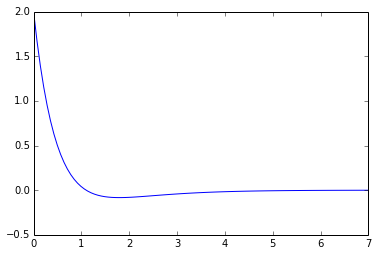
\includegraphics[max size={0.7\textwidth}{0.9\textheight}]{MRC_QUIGNONCHRISTOPHE_20140602_files/MRC_QUIGNONCHRISTOPHE_20140602_30_2.png}
\par
\end{center}

\end{codeoutput}

\end{codecell}

\textbf{Apply the inverse Laplace transform to each of the components of
the transfer function above. Create a function h(t) in Python, apply it
to the values of t obtained in the code snippet above and plot the
result. Compare the resulting plot to the plot above. Discuss the
result.}

\begin{codecell}


\begin{codeinput}
\begin{lstlisting}
# Answer 8.3.2
t = sympy.Symbol('t')
fun = (2*s + 1) / ((s + 1)*(s + 2))

sympy.pprint(inverse_laplace_transform(fun, s, t))

\end{lstlisting}
\end{codeinput}
\begin{codeoutput}


\begin{Verbatim}[commandchars=\\\{\}]
⎛ t    ⎞  -2*t             
-⎝e  - 3⎠*e    *Heaviside(t)
\end{Verbatim}

\end{codeoutput}

\end{codecell}

\begin{codecell}


\begin{codeinput}
\begin{lstlisting}
t, y = control.impulse_response(tf)
h = lambda _t: -(exp(t)-3)*exp(-2*_t)

plot(h(t))
show()
print 'Its the same!'
print 'Because the inverse laplace transform changes from s to time domain.'
\end{lstlisting}
\end{codeinput}
\begin{codeoutput}


\begin{center}
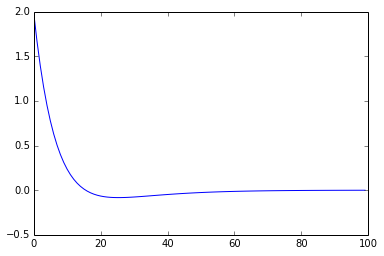
\includegraphics[max size={0.7\textwidth}{0.9\textheight}]{MRC_QUIGNONCHRISTOPHE_20140602_files/MRC_QUIGNONCHRISTOPHE_20140602_33_0.png}
\par
\end{center}

\begin{Verbatim}[commandchars=\\\{\}]
Its the same!
Because the inverse laplace transform changes from s to time domain.
\end{Verbatim}

\end{codeoutput}

\end{codecell}

\textbf{How to obtain the natural response of a system?}
\paragraph{Answer 8.3.3\ldots{}}


Now, take the transfer function as given above and gradually move the
pole at -1 closer and finally into the right half plane. What do you
notice?

\begin{enumerate}[1.]
\item
  How does this movement influence the behavior of the transfer
  function?
\item
  What can you say about how that affects the homogenous / natural
  response of the system?
\item
  Can you derive any criteria that would allow you to immediately
  characterize the behavior of a system / some important aspects of the
  system's behavior just by looking at the location of the poles and
  zeros, i.e.~it's pole/zero plot?
\end{enumerate}

# 1. If the poles are above zero, the system does not converge.
# 2. The poles define the homogeneous response.
#    The closer the pole get to zero, the faster the system convergesto its natural response.
# 3. A system is stable if the poles are below zero.

\begin{codecell}


\begin{codeinput}
\begin{lstlisting}
print 'pole up to 0:'
for i in  [1, 0.8, 0.6, 0.4, 0.2, 0.0]:
    #Factorized denominator:
    denom = control.series(control.tf([1, i], 1), control.tf( [1, 2], 1))
    tf = control.tf([2, 1], 1)/ denom
    #print tf
    plt.figure(0)
    control.pzmap.pzmap(tf)
    
    plt.figure(1)
    t, y = control.impulse_response(tf)
    plot(t, y, "b-")
show()

print 'pole above 0:'
for i in  [ 0.0, -0.2, -0.4, -.6, -.8 -1]:
    #Factorized denominator:
    denom = control.series(control.tf([1, i], 1), control.tf( [1, 2], 1))
    tf = control.tf([2, 1], 1)/ denom
    #print tf
    plt.figure(0)
    control.pzmap.pzmap(tf)

    plt.figure(1)
    t, y = control.impulse_response(tf)
    plot(t, y, "b-")
show()
print 'above zero, the system does not converge'
\end{lstlisting}
\end{codeinput}
\begin{codeoutput}


\begin{Verbatim}[commandchars=\\\{\}]
pole up to 0:
\end{Verbatim}

\begin{center}
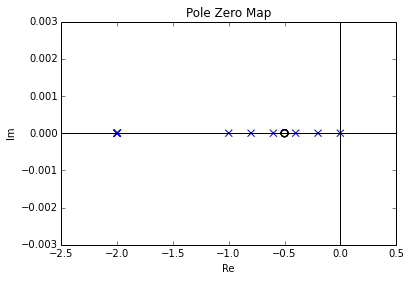
\includegraphics[max size={0.7\textwidth}{0.9\textheight}]{MRC_QUIGNONCHRISTOPHE_20140602_files/MRC_QUIGNONCHRISTOPHE_20140602_38_1.png}
\par
\end{center}

\begin{center}
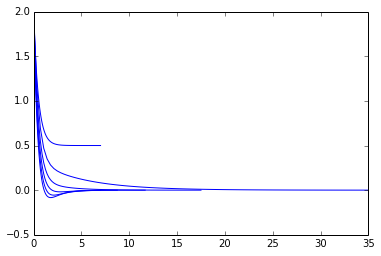
\includegraphics[max size={0.7\textwidth}{0.9\textheight}]{MRC_QUIGNONCHRISTOPHE_20140602_files/MRC_QUIGNONCHRISTOPHE_20140602_38_2.png}
\par
\end{center}

\begin{Verbatim}[commandchars=\\\{\}]
pole above 0:
\end{Verbatim}

\begin{center}
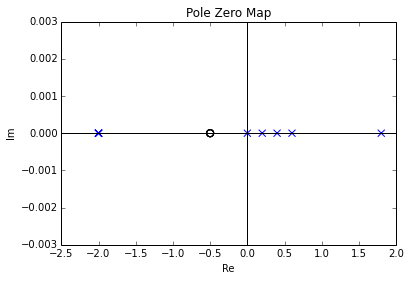
\includegraphics[max size={0.7\textwidth}{0.9\textheight}]{MRC_QUIGNONCHRISTOPHE_20140602_files/MRC_QUIGNONCHRISTOPHE_20140602_38_4.png}
\par
\end{center}

\begin{center}
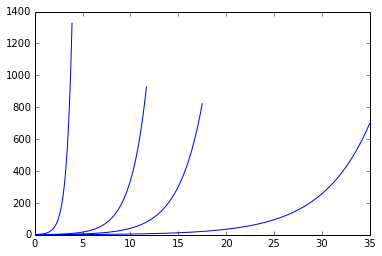
\includegraphics[max size={0.7\textwidth}{0.9\textheight}]{MRC_QUIGNONCHRISTOPHE_20140602_files/MRC_QUIGNONCHRISTOPHE_20140602_38_5.png}
\par
\end{center}

\begin{Verbatim}[commandchars=\\\{\}]
above zero, the system does not converge
\end{Verbatim}

\end{codeoutput}

\end{codecell}

\emph{Assignment 8.3 took me} \emph{minutes.}

\begin{center}\rule{3in}{0.4pt}\end{center}


\emph{Use this button to create a .txt file containing the time in
minutes you spent working on the assignments. Make sure to include your
name in the textbox below. The file will be created in the current
directory.}

Student's name:



\end{document}

